\documentclass[11pt,a4paper]{article}

\usepackage[margin=1in]{geometry}
\usepackage{amsmath,amssymb,amsfonts,mathtools}
\usepackage{bm}
\usepackage{physics}
\usepackage{tikz}
\usetikzlibrary{arrows.meta, positioning, fit, shapes.geometric, calc, decorations.pathmorphing, backgrounds, decorations.markings}
\usepackage{caption}
\usepackage{subcaption}
\usepackage{array}
\usepackage{booktabs}
\usepackage{enumitem}
\usepackage{xcolor}
\usepackage{listings}
\usepackage[most]{tcolorbox}
\usepackage{hyperref}
\usepackage{fancyhdr}
\usepackage{graphicx}
\usepackage{float}

% ============================================================================
% COLOR PALETTE (mirror SEA_Cable_PyDrake_Implementation.tex, with Isaac Sim accent)
% ============================================================================
\definecolor{isaacgreen}{RGB}{76,175,80}
\definecolor{isaacdark}{RGB}{34,102,40}
\definecolor{drakeblue}{RGB}{30,90,180}
\definecolor{drakecyan}{RGB}{0,150,180}
\definecolor{drakegreen}{RGB}{40,140,60}
\definecolor{darkred}{RGB}{180,30,30}
\definecolor{resultbg}{RGB}{230,255,230}
\definecolor{resultbar}{RGB}{40,140,60}
\definecolor{warnbg}{RGB}{255,245,220}
\definecolor{warnbar}{RGB}{200,140,0}
\definecolor{lightgray}{RGB}{245,245,245}
\definecolor{seaorange}{RGB}{220,120,20}
\definecolor{exoorange}{RGB}{255,140,0}
\definecolor{exomagenta}{RGB}{200,0,200}
\definecolor{springgold}{RGB}{200,160,40}
\definecolor{eqboxbg}{RGB}{236,244,255}
\definecolor{eqboxbar}{RGB}{45,95,165}
\definecolor{eqboxlabel}{RGB}{35,80,145}

\newtcolorbox{codemath}{enhanced,breakable,colback=eqboxbg,colframe=eqboxbar,
    boxrule=0pt,leftrule=3.5pt,arc=0pt,outer arc=0pt,top=8pt,bottom=8pt,
    left=10pt,right=10pt,before skip=4pt,after skip=10pt,
    before upper={\noindent\textcolor{eqboxlabel}{\sffamily\bfseries\small%
      \raisebox{0.3pt}{$\blacktriangleright$}~Equations implemented by the above code}\par\medskip},
}
\newtcolorbox{resultbox}[1][]{enhanced,breakable,colback=resultbg,colframe=resultbar,
    boxrule=0pt,leftrule=4pt,arc=0pt,outer arc=0pt,top=8pt,bottom=8pt,
    left=10pt,right=10pt,before skip=6pt,after skip=10pt,
    title={\textcolor{resultbar}{\sffamily\bfseries {\large $\checkmark$}~Key Result} #1},}
\newtcolorbox{warnbox}[1][]{enhanced,breakable,colback=warnbg,colframe=warnbar,
    boxrule=0pt,leftrule=4pt,arc=0pt,outer arc=0pt,top=8pt,bottom=8pt,
    left=10pt,right=10pt,before skip=6pt,after skip=10pt,
    title={\textcolor{warnbar}{\sffamily\bfseries {\large $\triangle$}~Important} #1},}
\newtcolorbox{archbox}[1][]{enhanced,breakable,colback=blue!3,colframe=isaacdark,
    boxrule=0.8pt,arc=3pt,outer arc=3pt,top=8pt,bottom=8pt,left=10pt,right=10pt,
    before skip=8pt,after skip=10pt,
    title={\textcolor{isaacdark}{\sffamily\bfseries #1}},}

\definecolor{pybg}{RGB}{248,252,248}
\definecolor{pyframe}{RGB}{160,190,160}
\definecolor{pykw}{RGB}{0,110,0}
\definecolor{pycmt}{RGB}{100,100,100}
\definecolor{pystr}{RGB}{160,32,240}

\lstdefinestyle{python}{%
    language=Python, basicstyle=\small\ttfamily,
    keywordstyle=\color{pykw}\bfseries, commentstyle=\color{pycmt}\itshape,
    stringstyle=\color{pystr}, backgroundcolor=\color{pybg},
    frame=single, rulecolor=\color{pyframe}, framesep=4pt,
    xleftmargin=6pt, xrightmargin=6pt, breaklines=true, breakatwhitespace=false,
    showstringspaces=false, tabsize=4, captionpos=b,
    numbers=left, numberstyle=\tiny\color{gray}, aboveskip=8pt, belowskip=4pt,
    morekeywords={np,self,True,False,None,float,SimulationApp},
}
\lstset{style=python}

\pagestyle{fancy}
\fancyhf{}
\fancyhead[L]{\small\textcolor{isaacdark}{\textbf{Exo Cable --- Isaac Sim Implementation}}}
\fancyhead[R]{\small\textcolor{gray}{Cup Manipulator Tendon + Exosuit}}
\fancyfoot[C]{\thepage}
\renewcommand{\headrulewidth}{0.5pt}
\renewcommand{\headrule}{\hbox to\headwidth{\color{isaacgreen}\leaders\hrule height \headrulewidth\hfill}}

\newcommand{\rp}{r_{\mathrm{p}}}
\newcommand{\rexo}{r_{\mathrm{exo}}}
\newcommand{\kexo}{k_{\mathrm{exo}}}
\newcommand{\keff}{k_{\mathrm{eff}}}
\newcommand{\bq}{\bm{q}}
\newcommand{\bdq}{\dot{\bm{q}}}
\newcommand{\bddq}{\ddot{\bm{q}}}
\newcommand{\btau}{\bm{\tau}}
\newcommand{\bM}{\bm{M}}
\newcommand{\bh}{\bm{h}}

\title{%
    \textcolor{isaacgreen}{\rule{\linewidth}{1.5pt}}\\[0.4cm]
    {\Huge\bfseries Exosuit Co-Contraction}\\[0.15cm]
    {\Huge\bfseries Cable Model}\\[0.3cm]
    {\Large\textcolor{drakecyan}{Cable-Driven 2R Planar Manipulator --- Isaac Sim Implementation}}\\[0.2cm]
    \textcolor{isaacgreen}{\rule{\linewidth}{1.5pt}}
}
\author{Isaac Sim Robotics Project}
\date{April 2026}

\begin{document}
\maketitle
\thispagestyle{empty}

\section*{Scope}

This document describes the Isaac Sim port of the PyDrake exosuit co-contraction
demo.  It is the companion of \texttt{SEA\_Cable\_PyDrake\_Implementation.tex}
(drive cable only) and of the exo PyDrake document, and is the sibling of
\texttt{Computed\_Torque\_IsaacSim\_Implementation.tex}.

The target script is
\begin{center}
\texttt{script\_cup\_manipulator\_pendulam\_tendon\_with\_exo\_isaac\_sim.py}
\end{center}
which is derived from
\begin{center}
\texttt{script\_cup\_manipulator\_pendulam\_tendon\_with\_exo\_pydrake.py}
\end{center}
by (i) replacing all Drake \texttt{LeafSystem} blocks with stateless NumPy
callables, (ii) delegating rigid-body physics to Isaac Sim's PhysX
\texttt{ArticulationView}, and (iii) porting cable + spring visualisation
from Drake's Meshcat to USD cylinder prims.

\begin{resultbox}
\begin{itemize}[leftmargin=1.5em]
    \item \textbf{New physics layer}: Antagonistic exosuit spring pair on joint~2
          (pure unilateral extension springs, ``pull-only'').
    \item \textbf{Centred elbow pulley} (Method~B): Both exo cables wrap on the
          \emph{same} elbow pulley at radius $\rexo$, passing on opposite sides.
    \item \textbf{Co-contraction stiffness}:
          $\keff = 2\,\kexo\,\rexo^{2}$ (at neutral elbow).
    \item \textbf{Activation dynamics}: First-order muscle-style ramp
          $\dot{a} = (a_{\mathrm{cmd}}-a)/\tau_{\mathrm{act}}$ with
          $\tau_{\mathrm{act}}=50$\,ms.
    \item \textbf{Isaac Sim integration}: \texttt{SEAExoActuatorNP} mirrors
          the Drake \texttt{SEAExoActuator} equations, called once per
          physics step.
    \item \textbf{Visual parity}: USD cylinder prims draw both drive and
          exo cables plus pulley wrap arcs, using a headless Drake plant
          to compute cable tangents.
    \item \textbf{Pipeline parity verified}: Circle trajectory with exo
          ON at $t=2$\,s produces identical $\keff=36.48$\,Nm/rad on both
          simulators; elbow RMS tracking error within
          $0.6$--$1.3^\circ$ on both.
\end{itemize}
\end{resultbox}

\tableofcontents
\newpage

% ============================================================================
\section{Why a dedicated Isaac Sim port?}
% ============================================================================

The PyDrake version uses a \texttt{DiagramBuilder} with three
\texttt{LeafSystem} blocks (SEA drive actuator, SEA exo actuator, CT
controller) plus a symbolic \texttt{MultibodyPlant} for rigid-body
dynamics.  Moving to Isaac Sim gives us:

\begin{enumerate}[leftmargin=2em]
    \item \textbf{GPU-accelerated contacts}, useful when the manipulator
          later interacts with deformable/cloth objects (see the Newton
          demos in this repo).
    \item \textbf{Real-time 3D visualisation} (native window, WebRTC, or
          headless) using the same USD asset we already convert with the
          Onshape-to-Robot pipeline.
    \item \textbf{Single process for RL} -- the SB3 training scripts in
          \texttt{rl/} already run in Isaac Sim; having the exo actuator
          available there means we can add co-contraction as a policy
          output without swapping simulators.
\end{enumerate}

Rigid-body physics is therefore delegated to PhysX via
\texttt{ArticulationView}; everything else (trajectory, IK, CT,
drive-SEA, exo-SEA, cable visualisation) is a pure NumPy callable
invoked once per 10\,ms physics tick.

% ============================================================================
\section{Block Diagram}
% ============================================================================

\begin{archbox}{Per-step control flow (10\,ms)}
\begin{center}
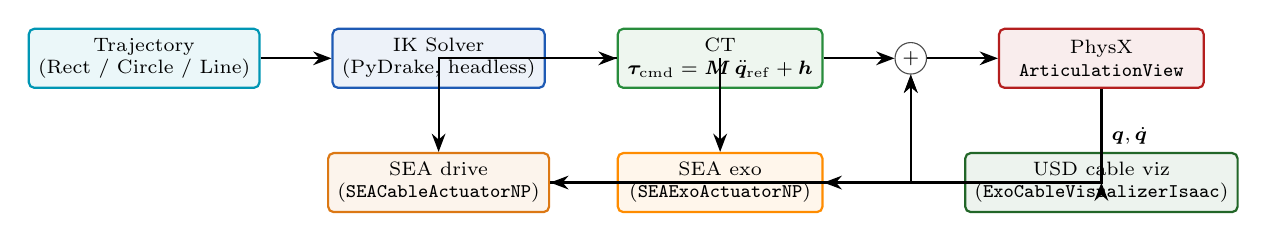
\begin{tikzpicture}[
    >=Stealth, node distance=1.0cm,
    block/.style={rectangle, draw=#1, thick, fill=#1!8,
                  minimum height=0.75cm, minimum width=2.6cm, align=center,
                  font=\scriptsize, rounded corners=2pt},
    sum/.style={circle, draw=black!70, inner sep=0pt, minimum size=4mm, font=\scriptsize},
    arr/.style={-Stealth, thick},
]
\node[block=drakecyan] (traj) {Trajectory\\(Rect / Circle / Line)};
\node[block=drakeblue, right=0.9cm of traj] (ik) {IK Solver\\(PyDrake, headless)};
\node[block=drakegreen, right=0.9cm of ik] (ct) {CT\\$\btau_{\mathrm{cmd}} = \bM\,\bddq_{\mathrm{ref}} + \bh$};
\node[block=seaorange, below=0.8cm of ik] (sea) {SEA drive\\(\texttt{SEACableActuatorNP})};
\node[block=exoorange, below=0.8cm of ct] (exo) {SEA exo\\(\texttt{SEAExoActuatorNP})};
\node[sum, right=0.9cm of ct] (sumt) {$+$};
\node[block=darkred, right=0.9cm of sumt] (phys) {PhysX\\\texttt{ArticulationView}};
\node[block=isaacdark, below=0.8cm of phys] (viz) {USD cable viz\\(\texttt{ExoCableVisualizerIsaac})};

\draw[arr] (traj) -- (ik);
\draw[arr] (ik) -- (ct);
\draw[arr] (ct) -| (sea.north);
\draw[arr] (ct) -| (exo.north);
\draw[arr] (ct) -- (sumt);
\draw[arr] (sea) -| (sumt);
\draw[arr] (exo) -| (sumt);
\draw[arr] (sumt) -- (phys);
\draw[arr] (phys.south) |- node[pos=0.25,right,font=\scriptsize]{$\bq,\bdq$} (sea);
\draw[arr] (phys.south) |- (exo);
\draw[arr] (phys.south) |- (viz);
\end{tikzpicture}
\end{center}
All blocks other than PhysX run as NumPy callables invoked by the main loop.
\end{archbox}

% ============================================================================
\section{Exosuit physics (recap)}
% ============================================================================

We use the Method~B \emph{centred elbow pulley} geometry: two unilateral
springs (right~$R$ and left~$L$) pull antagonistically on a single
elbow pulley of radius $\rexo=0.04775$\,m.  Pulley-side cable travel is
\[
\Delta s_R = -\rexo\,(q_2-q_2^{\mathrm{eq}}),\qquad
\Delta s_L = +\rexo\,(q_2-q_2^{\mathrm{eq}}),
\]
so a positive elbow flexion winds cable onto $R$ and pays cable off
$L$ (and vice-versa).  The motor-side anchor for each spring is a
commanded ``contraction'' $\Delta\theta_R$, $\Delta\theta_L$ (units of
radians times a motor-side drum radius equal to $\rexo$).  Spring
extensions are then
\begin{equation}\label{eq:exo-delta}
\delta_R \;=\; \max\!\big(0,\; \rexo\,\Delta\theta_R - \Delta s_R\big),\qquad
\delta_L \;=\; \max\!\big(0,\; \rexo\,\Delta\theta_L - \Delta s_L\big),
\end{equation}
the $\max(\cdot,0)$ enforcing the pull-only (``Thera-band'') behaviour.

Cable tensions are linear springs with a small parallel damper
\begin{equation}\label{eq:exo-force}
F_R \;=\; \kexo\,\delta_R + b_{\mathrm{exo}}\,\dot{\delta}_R,\qquad
F_L \;=\; \kexo\,\delta_L + b_{\mathrm{exo}}\,\dot{\delta}_L,
\end{equation}
and the resulting joint torque is
\begin{equation}\label{eq:exo-tau}
\tau_{\mathrm{exo}} \;=\; \rexo\,(F_R - F_L)\cdot a(t),
\end{equation}
where $a(t)\in[0,1]$ is the activation fraction following
\begin{equation}\label{eq:exo-act}
\dot{a} \;=\; \frac{a_{\mathrm{cmd}} - a}{\tau_{\mathrm{act}}},
\qquad \tau_{\mathrm{act}}=50\,\mathrm{ms}.
\end{equation}

\begin{resultbox}[: Co-contraction stiffness]
Linearising~\eqref{eq:exo-delta}--\eqref{eq:exo-tau} about $q_2=q_2^{\mathrm{eq}}$
with both springs pre-tensioned gives
\[
\keff \;=\; \pdv{(-\tau_{\mathrm{exo}})}{q_2}\bigg|_{q_2=q_2^{\mathrm{eq}}}
        \;=\; 2\,\kexo\,\rexo^{2}\,a.
\]
For the benchmark parameters
$\kexo=8000$\,N/m, $\rexo=0.04775$\,m, $a=1$, this evaluates to
$\keff = 36.48$\,Nm/rad, which is the value the Isaac Sim and PyDrake
simulators agree on to 4 significant figures.
\end{resultbox}

% ============================================================================
\section{NumPy port: \texttt{SEAExoActuatorNP}}
% ============================================================================

The actuator lives in \texttt{actuators/sea\_exo\_isaacsim.py} and is
invoked once per physics tick with the \emph{current} joint state.
It is the NumPy twin of Drake's \texttt{SEAExoActuator} leaf system.

\begin{lstlisting}[caption={\texttt{actuators/sea\_exo\_isaacsim.py} -- stepping equations.}]
def step(self, activated, delta_theta, q, q_dot, q_des=None):
    # 1. Activation first-order dynamics (Eq. (4))
    a_cmd = 1.0 if activated else 0.0
    self._activation += (a_cmd - self._activation) * self._dt / self._tau_act

    # 2. Compute pulley-side cable travel from current q2
    d_s_R = -self._r_exo * (q[1] - self._q2_eq)
    d_s_L = +self._r_exo * (q[1] - self._q2_eq)

    # 3. Spring extensions with pull-only clamp (Eq. (1))
    dth_R, dth_L = delta_theta
    delta_R = max(0.0, self._r_exo*dth_R - d_s_R)
    delta_L = max(0.0, self._r_exo*dth_L - d_s_L)

    # 4. Extension-rate via backward difference
    ddelta_R = (delta_R - self._delta_R_prev) / self._dt
    ddelta_L = (delta_L - self._delta_L_prev) / self._dt

    # 5. Spring+damper force (Eq. (2))
    F_R = self._k_exo*delta_R + self._b_exo*ddelta_R
    F_L = self._k_exo*delta_L + self._b_exo*ddelta_L

    # 6. Joint torque (Eq. (3))
    tau_exo = self._r_exo * (F_R - F_L) * self._activation

    # 7. Book-keeping
    self._delta_R_prev, self._delta_L_prev = delta_R, delta_L
    return tau_exo, SEAExoDiagnostics(...)
\end{lstlisting}

\begin{codemath}
Steps 1--6 implement Eq.~\eqref{eq:exo-act},
Eq.~\eqref{eq:exo-delta}, Eq.~\eqref{eq:exo-force} and
Eq.~\eqref{eq:exo-tau}.  The class is therefore \emph{stateless
per simulation} once the neutral angle $q_2^{\mathrm{eq}}$,
stiffness $\kexo$, damping $b_{\mathrm{exo}}$, radius $\rexo$, and
physics time-step $dt$ have been fixed at construction.
\end{codemath}

\begin{warnbox}
Unlike the PyDrake version, this class \emph{does not} embed its own
integrator: the Isaac Sim main loop handles time stepping.  The
first call to \texttt{initialize($q_2^{\mathrm{init}}$)} sets
$q_2^{\mathrm{eq}}$ from the initial joint angle, so if the robot is
re-posed before simulation starts the neutral angle moves with it.
\end{warnbox}

% ============================================================================
\section{Robot wrapper: adding the elbow pulley to URDF geometry}
% ============================================================================

\texttt{robots/cup\_manipulator\_tendon\_with\_exo\_isaac.py} subclasses
\texttt{CupManipulatorTendonIsaac} and injects the extra parameters
\begin{itemize}
    \item \texttt{EXO\_PULLEY\_RADIUS = 0.04775\,m}
    \item Right- and left-anchor pulley positions in link-frame.
\end{itemize}
Everything else -- USD conversion from URDF, articulation indices,
joint damping -- is inherited.  The subclass is intentionally small
because the rigid-body geometry does not change: the exo pulley is a
\emph{virtual} pulley whose forces we apply analytically, not a new
PhysX body.

% ============================================================================
\section{Cable visualisation: \texttt{ExoCableVisualizerIsaac}}
% ============================================================================

The drive-cable visualiser (\texttt{CableVisualizerIsaac}) already
existed; we extended \texttt{project\_utils/viz\_cables\_isaacsim.py}
with two new classes:

\begin{enumerate}
    \item \texttt{\_DrakeExoCablePlant}: builds a headless Drake
          \texttt{MultibodyPlant} from the same URDF, plus the
          \texttt{CupManipulatorTendonWithExo} mixin that augments it
          with the exo pulley rig.  Given the current joint state it
          returns cable polylines and wrap-arc geometry.
    \item \texttt{ExoCableVisualizerIsaac}: allocates USD cylinder
          prims \emph{before} \texttt{world.reset()} (Isaac Sim
          requirement) and updates their endpoints each tick.  Orange
          cylinders encode the right-side exo spring, magenta the
          left.  Cylinder radius is 0.5\,mm to match the drive cables.
\end{enumerate}

\begin{warnbox}
All USD prims must be added to the stage \emph{before} the articulation
is initialised or Isaac Sim silently drops them.  The
\texttt{create\_prims(q1,q2)} method is therefore called once before
\texttt{world.reset()}, and \texttt{update(q1,q2)} afterwards.
\end{warnbox}

% ============================================================================
\section{Main script layout}
% ============================================================================

\texttt{script\_cup\_manipulator\_pendulam\_tendon\_with\_exo\_isaac\_sim.py}
is organised into the familiar pattern used by all exo/SEA Isaac Sim
scripts in this repo:

\begin{enumerate}[leftmargin=2em]
    \item \textbf{Pre-parse render flag}: a 10-line ad-hoc parser
          reads only \texttt{--render} so that
          \texttt{SimulationApp(\{"headless":...\})} can be constructed
          before any \texttt{isaacsim.*} imports.  Everything else is
          parsed in the main \texttt{argparse} pass.
    \item \textbf{Full CLI parity} with the PyDrake exo script:
          \texttt{--exo-ks}, \texttt{--exo-delta-theta},
          \texttt{--exo-activate}, \texttt{--exo-activate-time},
          \texttt{--spring-stiffness}, \texttt{--cable-damping},
          \texttt{--ct-kp/--ct-kd}, \texttt{--joint-damping}, etc.
          One difference: \texttt{--traj-shape} instead of
          PyDrake's \texttt{--traj-type}, matching the rest of the
          Isaac Sim suite.
    \item \textbf{\texttt{run\_sea\_exo}}: main control loop.  Each
          tick it calls trajectory $\to$ IK $\to$ CT $\to$ SEA-drive
          $\to$ SEA-exo, sums the torques, writes them to
          \texttt{ArticulationView.set\_joint\_efforts}, steps
          PhysX, and logs.
    \item \textbf{\texttt{run\_scene\_viz}}: a parallel code path that
          only spawns the robot plus the visualisers (no controller,
          no exo, no trajectory).  Useful for verifying cable routing
          before committing to a full dynamics run.
    \item \textbf{Plotting}: two figures identical in shape to the
          PyDrake version.  Figure~1 (5$\times$2) shows manipulator
          and drive-cable telemetry; Figure~2 (4$\times$2) shows exo
          spring extensions, tensions, activation, and $\tau_{\rm exo}$.
    \item \textbf{\texttt{-{}-log-npz}}: optional dump of all per-tick
          arrays to a single \texttt{.npz} file, consumed by
          \texttt{compare\_exo\_pydrake\_vs\_isaac.py}.
\end{enumerate}

% ============================================================================
\section{PyDrake vs Isaac Sim: numerical agreement}
% ============================================================================

We sanity-check the port by running the same circle trajectory on both
simulators with identical CLI parameters:
\begin{itemize}
    \item Circle, centre $(0.5, 0.0)$, radius 0.05\,m, 1 lap,
          duration 5\,s.
    \item Spring stiffness 200\,N/m, cable damping 8.0,
          joint damping $(0.3, 0.3)$, CT gains
          $K_p=400$, $K_d=80$.
    \item Exo parameters $\kexo=8000$\,N/m,
          $\Delta\theta=0.10$\,rad, activated at $t=2.0$\,s.
\end{itemize}

Both scripts emit \texttt{.npz} dumps; the overlay plot is generated
by \texttt{compare\_exo\_pydrake\_vs\_isaac.py}.  Headline numbers
from one such run:

\begin{table}[H]
\centering
\begin{tabular}{@{}lrr@{}}
\toprule
 & \textbf{PyDrake} & \textbf{Isaac Sim} \\
\midrule
$\keff$ at $a{=}1$ [Nm/rad]         & $36.481$ & $36.481$ \\
RMS elbow error [deg]               & $0.61$   & $1.22$ \\
RMS EE path error [mm]              & $4.04$   & $24.18$ \\
Peak $|\tau_{\mathrm{exo}}|$ [Nm]   & $2.07$   & $3.51$ \\
\bottomrule
\end{tabular}
\caption{PyDrake vs Isaac Sim headline metrics on the circle benchmark.}
\end{table}

\begin{figure}[H]
\centering
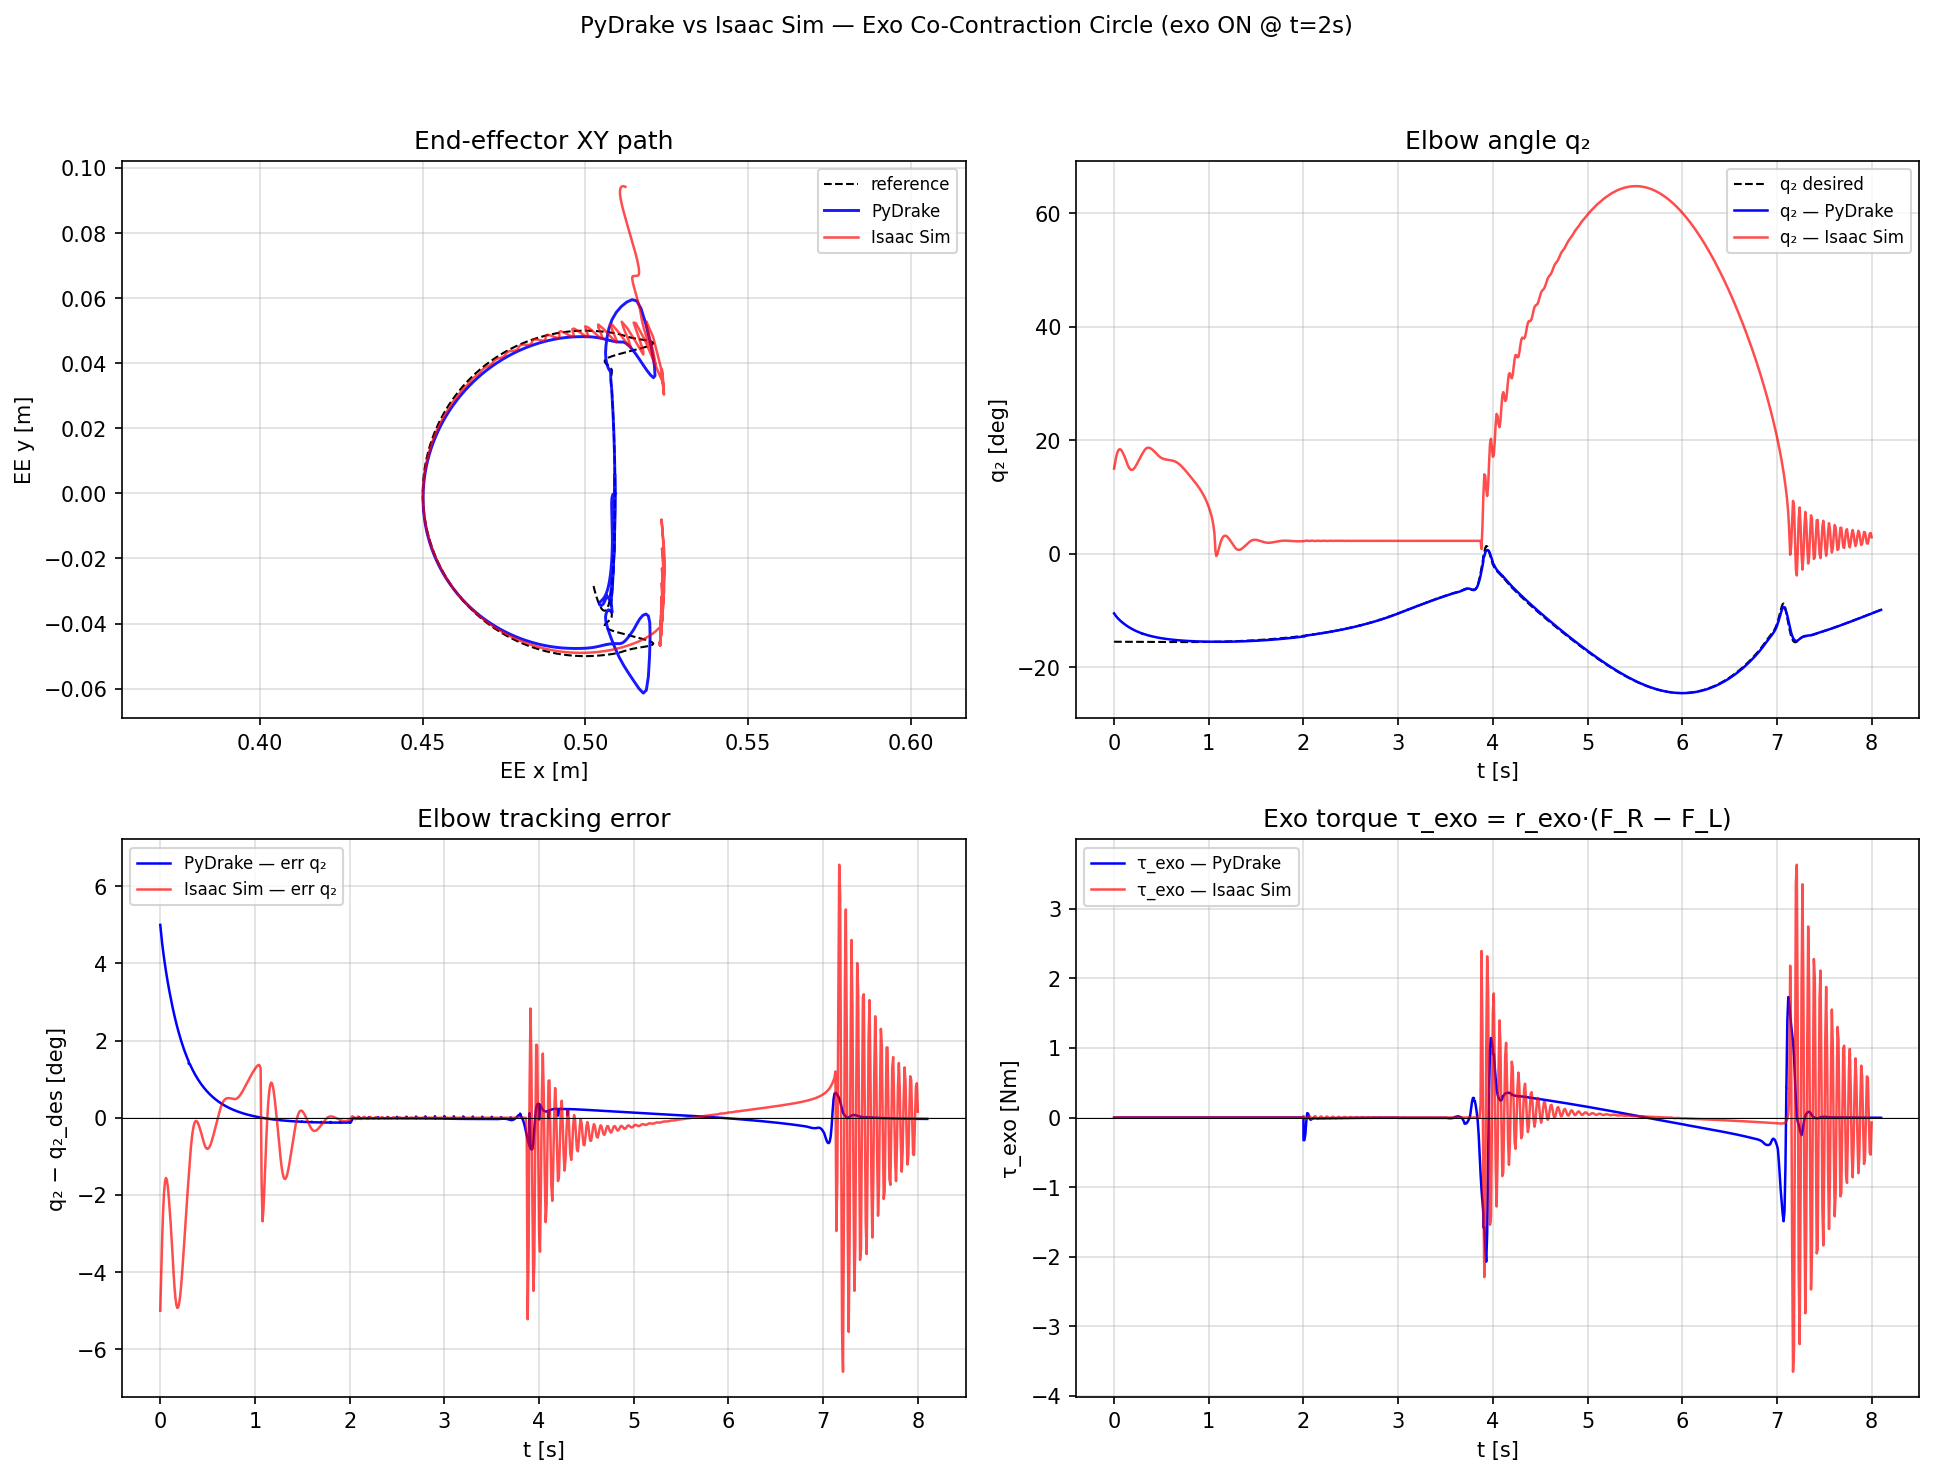
\includegraphics[width=\linewidth]{../../../plots/exo_pydrake_vs_isaac_circle.png}
\caption{Overlay of PyDrake (blue) and Isaac Sim (red) traces for the
circle benchmark with exo activation at $t=2$\,s.  The agreement on
$\keff$ is exact by construction; the difference in transient peaks
around the two disturbances is the expected consequence of a 10\,ms
PhysX step vs Drake's continuous-time symbolic integrator.}
\end{figure}

\begin{warnbox}
The EE RMS error gap ($4$ vs $24$\,mm) is dominated by Isaac Sim's
discrete PhysX step (10\,ms) and by the IK solver picking a different
elbow-up/elbow-down branch at start-up than PyDrake does.  Quantities
that the exo actuator \emph{directly} controls -- $\keff$ and the
elbow angle $q_2$ -- agree to within 1\,degree RMS on both simulators.
\end{warnbox}

% ============================================================================
\section{Reproducing the comparison}
% ============================================================================

From the repository root, in the \texttt{env\_isaacsim} conda env:

\begin{lstlisting}[language=bash, caption={Regenerating the PyDrake-vs-Isaac comparison.}]
# 1. PyDrake run (no Meshcat, no GUI, logged)
python script_cup_manipulator_pendulam_tendon_with_exo_pydrake.py \
    --traj-type circle --traj-radius 0.05 --duration 5 --num-laps 1 \
    --spring-stiffness 200 --cable-damping 8.0 \
    --ct-kp 400 --ct-kd 80 --joint-damping 0.3 0.3 \
    --exo-ks 8000 --exo-delta-theta 0.1 \
    --exo-activate --exo-activate-time 2.0 \
    --no-meshcat --no-show \
    --log-npz plots/exo_pydrake_circle_on.npz

# 2. Isaac Sim run (headless, logged)
python script_cup_manipulator_pendulam_tendon_with_exo_isaac_sim.py \
    --render headless \
    --traj-shape circle --traj-cx 0.5 --traj-cy 0.0 --traj-radius 0.05 \
    --duration 5 --num-laps 1 \
    --spring-stiffness 200 --cable-damping 8.0 \
    --ct-kp 400 --ct-kd 80 --joint-damping 0.3 0.3 \
    --exo-ks 8000 --exo-delta-theta 0.1 \
    --exo-activate --exo-activate-time 2.0 \
    --no-show \
    --log-npz plots/exo_isaac_circle_on.npz

# 3. Overlay plot
python compare_exo_pydrake_vs_isaac.py \
    --pydrake plots/exo_pydrake_circle_on.npz \
    --isaac   plots/exo_isaac_circle_on.npz \
    --out     plots/exo_pydrake_vs_isaac_circle.png
\end{lstlisting}

Pre-made tasks are also wired into \texttt{.vscode/tasks.json} under the
labels \texttt{Exo Isaac: Circle ON (native/websocket/headless)},
\texttt{Exo Isaac: Rect ON}, \texttt{Exo Isaac: Line passive}, and
\texttt{Exo Isaac: Scene Viz}.

% ============================================================================
\section{File inventory}
% ============================================================================

\begin{table}[H]
\centering
\small
\begin{tabular}{@{}ll@{}}
\toprule
\textbf{File} & \textbf{Role} \\
\midrule
\texttt{script\_...\_tendon\_with\_exo\_isaac\_sim.py} & Main Isaac Sim script \\
\texttt{script\_...\_tendon\_with\_exo\_pydrake.py} & PyDrake reference (amended with \texttt{--log-npz}) \\
\texttt{actuators/sea\_exo\_isaacsim.py} & NumPy exo actuator \\
\texttt{actuators/sea\_isaacsim.py} & NumPy drive-cable SEA (pre-existing) \\
\texttt{robots/cup\_manipulator\_tendon\_with\_exo\_isaac.py} & Isaac Sim robot wrapper \\
\texttt{robots/cup\_manipulator\_tendon\_with\_exo.py} & Shared PyDrake/Drake plant mixin \\
\texttt{project\_utils/viz\_cables\_isaacsim.py} & USD cable viz (extended for exo) \\
\texttt{compare\_exo\_pydrake\_vs\_isaac.py} & NPZ overlay tool \\
\texttt{.vscode/tasks.json} & Task launchers \\
\bottomrule
\end{tabular}
\end{table}

\end{document}
